\documentclass[11pt,answers]{exam}

\usepackage{etex}
\usepackage{amssymb,amsmath,multicol} %<-- InWorksheetExam1 i also have fancyhdr,

\usepackage[metapost]{mfpic}
\usepackage[pdftex]{graphicx}

\usepackage{pst-plot}
\usepackage{pgfplots}
\pgfplotsset{compat=1.9}

\usepackage{tikz}
\usepackage{tkz-2d}
\usepackage{tkz-base}
\usetikzlibrary{calc}

\usepackage[inline]{enumitem}
\usepackage{refcount}%<-- non in WorksheetExam1

\usepackage{pstricks-add,pst-eucl}

\def\f{x+1} \def\g{-x/3+2}  \def\h{-x+3}

\newcommand{\vasymptote}[2][]{
    \draw [densely dashed,#1] ({rel axis cs:0,0} -| {axis cs:#2,0}) -- ({rel axis cs:0,1} -| {axis cs:#2,0});
}

\addpoints
%\printanswers
\noprintanswers

\opengraphsfile{Q1a_Spring_16}

\begin{document}
\extrawidth{-0.3in}
\pagestyle{headandfoot}

\setlength{\hoffset}{-.25in}

\extraheadheight{-.3in}
\runningheadrule
\firstpageheader{\bfseries {MATH1-UC 1171}}{ \bfseries {Quiz 1 }}{\bfseries {2/2/16}} 



\firstpagefooter{} %%&&CHANGED
                {}
                {Points earned: \hbox to 0.5in{\hrulefill}
                 out of  \pointsonpage{\thepage} points}
                 
						

\vspace*{0.1cm}
\hbox to \textwidth { \scshape {Name:} \enspace\hrulefill}
\vspace{0.1in}




\pointpoints{point}{points}

\begin{questions}


\addpoints

\bonusquestion[1]  Write a system of two linear equations in two unknowns that has no solutions.

\fillwithdottedlines{2cm}



\question[4] 

The shaded region in the graph shown below represents a feasible region.

\begin{minipage}{0.5\linewidth}
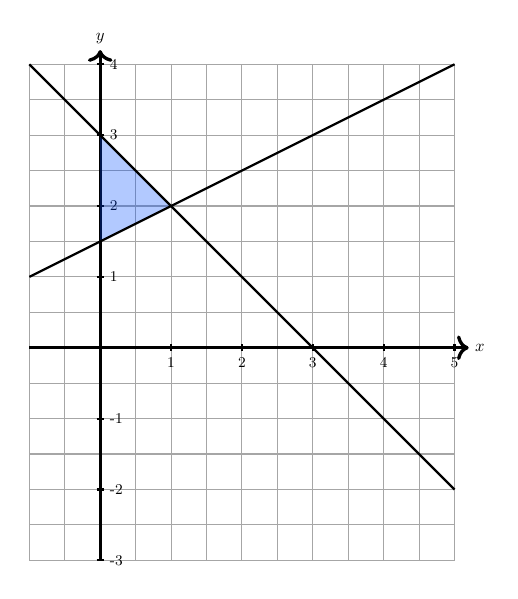
\begin{tikzpicture}[thick,scale=0.9, every node/.style={scale=0.6}]

    \draw[gray!70, thin, step=0.5] (-1,-3) grid (5,4);
    \draw[very thick,->] (-1,0) -- (5.2,0) node[right] {$x$};
    \draw[very thick,->] (0,-3) -- (0,4.2) node[above] {$y$};

    \foreach \x in {1,...,5} \draw (\x,0.05) -- (\x,-0.05) node[below] {\small\x};
    \foreach \y in {1,...,4} \draw (-0.05,\y) -- (0.05,\y) node[right] {\small\y};
    \foreach \y in {-3,...,-1} \draw (-0.05,\y) -- (0.05,\y) node[right] {\small\y};

    \fill[blue!70!cyan,opacity=0.3] (0,3/2) -- (1,2) -- (0,3) -- cycle;

    \draw (-1,4) -- node[below,sloped] {} (5,-2);
    %\draw (1,-3) -- (3,1) -- node[below left,sloped] {} (4.5,4);
    \draw (-1,1) -- node[above,sloped] {} (5,4);

\end{tikzpicture} 
\end{minipage}
\begin{minipage}{0.5\linewidth}
 Write a system of three inequalities that has the region as its solution set. Show your work step-by-step and box each inequality.
\fillwithdottedlines{0.25\textheight}
\end{minipage}



\fillwithdottedlines{3cm}
\question[4] Translate this description into a system of linear inequalities, setting $x$ to be the number of chairs and $y$ the number of tables. {\em{A furniture manufacturer makes wooden tables and chairs. The production process involves two basic types of labor: carpentry and finishing. A table requires 2 hours of carpentry and 1 hour of finishing, and a chair requires 3 hours of carpentry and half an hour of finishing. The manufacturer's employees can supply a maximum of 108 hours of carpentry work and a maximum of 20 hours of finishing work per day.}} Box each inequality and do not graph the solution set.
\fillwithdottedlines{3.5cm}


%%%%%%%%%%%%%%%%%%%%%%%%%%



\end{questions}

\end{document}                 